\chapter{Priprava na 1. laboratorijske vaje}

\section{Boolova algebra in preklopne funkcije}

Preklopne (tudi logične) funkcije so funkcije nad preklopnimi (tudi logičnimi) spremenljivkami (spremenljivke, ki lahko zavzamejo vrednosti iz množice $\left\{0, 1\right\}$) in nad katerimi temelji procesiranje podatkov z uporabo digitalnih vezij. Preklopne funkcije (operatorji), elementi nad katerimi operirajo (operandi) in pravila po katerih operirajo so definirani z Boolovo algebro.

Boolovo algebro lahko definiramo kot trojček $\left\{X, O, P\right\}$, kjer je $X$ množica elementov Boolove algebre (operandov), $O$ množica osnovnih funkcij (operatorjev), ki vsebuje disjunkcijo ($\vee$) in konjunkcijo ($\cdot$), in $P$ množica postulatov oziroma pravil, ki so opisana v nadaljevanju.

\subsection{Postulati Boolove algebre}
\subsubsection*{Zaprtost}
\begin{align*}
\texttt{P1}&\texttt{:}x,y \in X; x \vee y \in X\\
\texttt{P1}^*&\texttt{:}x,y \in X; x \cdot y \in X
\end{align*}

\subsubsection*{Nevtralni element}
\begin{align*}
\texttt{P2}&\texttt{:}x,0 \in X; x \vee 0 = x\\
\texttt{P2}^*&\texttt{:}x,1 \in X; x \cdot 1 = x
\end{align*}

\subsubsection*{Komutativnost}
\begin{align*}
\texttt{P3}&\texttt{:}x,y \in X; x \vee y = y \vee x\\
\texttt{P3}^*&\texttt{:}x,y \in X; x \cdot y = y \cdot x
\end{align*}

\subsubsection*{Distributivnost}
\begin{align*}
\texttt{P4}&\texttt{:}x,y,z \in X; x \vee \left(y \cdot z \right) = \left(x \vee y\right) \cdot \left( x \vee z\right)\\
\texttt{P4}^*&\texttt{:}x,y,z \in X; x \cdot \left(y \vee z \right) = \left(x \cdot y\right) \vee \left( x \cdot z\right)
\end{align*}

\subsubsection*{Inverzni element}
\begin{align*}
\texttt{P5}&\texttt{:}\forall x \in X, \exists \ol x \in X; x \vee \ol x = 1\\
\texttt{P5}^*&\texttt{:}\forall x \in X, \exists \ol x \in X; x \cdot \ol x = 0
\end{align*}

\subsubsection*{Število elementov}
\begin{align*}
\texttt{P6}&\texttt{:}\exists x,y \in X; x \neq y
\end{align*}

\subsection{Lastnosti Boolove algebre}
Iz postulatov izhajajo določene lastnosti, ki jih lahko uporabimo pri poenostavljanju logičnih izrazov. V nadaljevanju je naštetih nekaj bolj uporabnih lastnosti.
\subsubsection*{Idempotenca}
\begin{align*}
x \vee x \vee \dots \vee x = x\\
x \cdot x \cdot \dots \cdot x = x
\end{align*}

\subsubsection*{Absorpcija}
\begin{align*}
x \vee x \cdot y = x\\
x \cdot \left( x \vee y\right) = x
\end{align*}

\subsubsection*{Asociativnost}
\begin{align*}
\left(x \vee y \right)\vee z = x \vee \left(y \vee z \right)= x \vee y \vee z\\
\left(x \cdot y \right)\cdot z = x \cdot \left(y \cdot z \right)= x \cdot y \cdot z
\end{align*}

\subsubsection*{DeMorganovo pravilo}
\begin{align*}
\ol{\left(x_1 \vee x_2 \vee \dots \vee x_n \right)} = \ol x_1 \cdot \ol x_2 \cdot \dots \cdot \ol x_n\\
\ol{\left(x_1 \cdot x_2 \cdot \dots \cdot x_n \right)} = \ol x_1 \vee \ol x_2 \vee \dots \vee \ol x_n
\end{align*}



\section{Podajanje preklopnih funkcij}
Vsako preklopno funkcijo lahko podamo na različne načine, pri čemer so osnovni načini sledeči:
\begin{itemize}
\item \emph{Logični izraz} funkcijo podaja analitično, tj. kot enačbo, v kateri nastopajo logične spremenljivke (operandi), ki so med seboj povezane preko preklopnih funkcij (operatorji).
\item \emph{Logična shema} funkcijo podaja grafično, tj.  s shemo njene realizacije. Vhodi v shemo opisujejo vhodne spremenljivke, izhodi iz sheme pa izhodne. V shemi uporabljamo logične simbole, ki predstavljajo osnovne logične operatorje (opozorilo: v različni literaturi boste srečali različne logične simbole).
\item \emph{Pravilnostna tabela} funkcijo podaja tabelarično, tj. podaja vse možne kombinacije vhodnih vektorjev in funkcijske vrednosti pri posamezni kombinaciji. Pri tem na levi strani tabele nastopajo vhodne (neodvisne) spremenljivke, ki določajo vhodni vektor, na desni pa izhodne (odvisne) spremenljivke. Poljubno preklopno funkcijo z $n$ vhodnimi spremenljivkami lahko opišemo s pravilnostno tabelo, ki ima $2^n$ vrstic.
\item \emph{Veitchevega diagrama} zaenkrat še ne bomo podrobneje obravnavali.
\end{itemize}

\section{Osnovne preklopne funkcije}
Boolova algebra definira osnovna logična operatorja, tj. disjunkcijo (or) in konjunkcijo (and). Preko postulata \emph{Inverzni element} vpeljemo še negacijo (not). V nadaljevanju podajamo osnovne logične operatorje, s katerimi lahko zapišemo poljubno preklopno funkcijo in so realizirani tudi znotraj družine logičnih čipov 7400. 

\subsection{Disjunkcija}

Disjunkcija (ALI, OR) vrne logično 1, ko je na logično 1 postavljena vsaj ena izmed njenih vhodnih spremenljivk. V logičnem izrazu jo označujemo s simbolom $\vee$. Slika \ref{fig:or} podaja logični izraz (a), logični simbol (b) in pravilnostno tabelo (c) za disjunkcijo z dvema vhodnima spremenljivkama.


\begin{figure}[ht]
\begin{center}
\begin{tabular}{ccc}
$y = x_1 \vee x_2$&

\includegraphics{or.eps}&
\begin{tabular}{cc|c}
$x_1$ & $x_2$ & $y$\\
\hline
$0$ & $0$ & $0$\\
$0$ & $1$ & $1$\\
$1$ & $0$ & $1$\\
$1$ & $1$ & $1$
\end{tabular}\\
(a) & (b) & (c)
\end{tabular}	
\caption{Logični izraz (a), logični simbol (b) in pravilnostna tabela (c) za disjunkcijo z dvema vhodnima spremenljivkama.}
\label{fig:or}
\end{center}
\end{figure}


\subsection{Konjunkcija}
Konjunkcija (IN, AND) vrne logično 1, ko so na logično 1 postavljene vse vhodne spremenljivke.  V logičnem izrazu jo označujemo s simbolom $\wedge$ ali $\cdot$, včasih pa simbol celo izpustimo (podobno kot pri množenju). Slika \ref{fig:and} podaja logični izraz (a), logični simbol (b) in pravilnostno tabelo (c) za konjunkcijo z dvema vhodnima spremenljivkama.

\begin{figure}[ht]
\begin{center}
\begin{tabular}{ccc}
$y = x_1 \cdot x_2 = x_1 x_2$ &

\includegraphics{and.eps}&
\begin{tabular}{cc|c}
$x_1$ & $x_2$ & $y$\\
\hline
$0$ & $0$ & $0$\\
$0$ & $1$ & $0$\\
$1$ & $0$ & $0$\\
$1$ & $1$ & $1$
\end{tabular}\\
(a) & (b) & (c)
\end{tabular}	
\caption{Logični izraz (a), logični simbol (b) in pravilnostna tabela (c) za konjunkcijo z dvema vhodnima spremenljivkama.}
\label{fig:and}
\end{center}
\end{figure}

\subsection{Negacija}
Negacija (NE, NOT) invertira vhodno logično spremenljivko. V logičnem izrazu jo označujemo s črto nad vhodno spremenljivko. Slika \ref{fig:not} podaja logični izraz (a), logični simbol (b) in pravilnostno tabelo (c) za negacijo.

\begin{figure}[ht]
\begin{center}
\begin{tabular}{ccc}
$y = \ol x$&
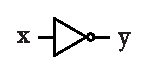
\includegraphics{not.eps}&
\begin{tabular}{c|c}
$x$ & $y$\\
\hline
$0$ & $1$\\
$1$ & $0$
\end{tabular}\\
(a) & (b) & (c)
\end{tabular}	
\caption{Logični izraz (a), logični simbol (b) in pravilnostna tabela (c) za negacijo.}
\label{fig:not}
\end{center}
\end{figure}


\subsection{Peircov operator}

Peircov operator (NE ALI, NOR) predstavlja invertirano (negirano) disjunkcijo. Operator vrne logično 1, ko so na logično 0 postavljene vse vhodne spremenljivke. V logičnem izrazu ga označujemo s simbolom $\downarrow$. Slika \ref{fig:nor} podaja logični izraz (a), logični simbol (b) in pravilnostno tabelo (c) za Peircov operator z dvema vhodnima spremenljivkama.

\begin{figure}[ht]
\begin{center}
\begin{tabular}{ccc}
$y = x_1 \downarrow x_2  = \ol{\left( x_1 \vee x_2 \right)}$&

\includegraphics{nor.eps}&
\begin{tabular}{cc|c}
$x_1$ & $x_2$ & $y$\\
\hline
$0$ & $0$ & $1$\\
$0$ & $1$ & $0$\\
$1$ & $0$ & $0$\\
$1$ & $1$ & $0$
\end{tabular}\\
(a) & (b) & (c)
\end{tabular}	
\caption{Logični izraz (a), logični simbol (b) in pravilnostna tabela (c) za Peircov operator z dvema vhodnima spremenljivkama.}
\label{fig:nor}
\end{center}
\end{figure}

Opozorilo: asociativnost za Peircov operator ne velja: $x_1 \downarrow x_2 \downarrow x_3 \neq \left( x_1 \downarrow x_2 \right) \downarrow x_3 \neq x_1 \downarrow \left(x_2 \downarrow x_3\right)$!

\subsection{Shefferjev operator}
Shefferjev operator (NE IN, NAND) predstavlja invertirano (negirano) konjunkcijo. Operator vrne logično 0, ko so na logično 1 postavljene vse vhodne spremenljivke. V logičnem izrazu ga označujemo s simbolom $\uparrow$. Slika \ref{fig:nor} podaja logični izraz (a), logični simbol (b) in pravilnostno tabelo (c) za Shefferjev operator z dvema vhodnima spremenljivkama.

\begin{figure}[ht]
\begin{center}
\begin{tabular}{ccc}
$y = x_1 \uparrow x_2 = \ol{\left( x_1 x_2 \right)}$&

\includegraphics{nand.eps}&
\begin{tabular}{cc|c}
$x_1$ & $x_2$ & $y$\\
\hline
$0$ & $0$ & $1$\\
$0$ & $1$ & $1$\\
$1$ & $0$ & $1$\\
$1$ & $1$ & $0$
\end{tabular}\\
(a) & (b) & (c)
\end{tabular}	
\caption{Logični izraz (a), logični simbol (b) in pravilnostna tabela (c) za Shefferjev operator z dvema vhodnima spremenljivkama.}
\label{fig:nand}
\end{center}
\end{figure}

Opozorilo: asociativnost za Shefferjev operator ne velja: $x_1 \uparrow x_2 \uparrow x_3 \neq \left( x_1 \uparrow x_2 \right) \uparrow x_3 \neq x_1 \uparrow \left(x_2 \uparrow x_3\right)$!

\subsection{Ekskluzivni ali}
Ekskluzivni ali (XOR, tudi vsota po modulu 2) dveh vhodnih spremenljivk vrne logično 1, ko logično vrednost 1 ekskluzivno zavzema ena vhodna spremenljivka. Pri več vhodnih spremenljivkah funkcija vrne logično 1, ko je na logično vrednost 1 postavljenih liho število vhodnih spremenljivk, kar si lahko interpretiramo tudi kot vsota po modulu 2 (opozorilo: v Logisimu XOR privzeto ne deluje na tak način -- pod lastnostmi XOR vrat moramo nastaviti polje \emph{Multiple-Input Behavior} na vrednost \emph{When an odd number are on}). V logičnem izrazu ekskluzivni ALI označujemo s simbolom $\nabla$ ali $\oplus$. Slika \ref{fig:xor} podaja logični izraz (a), logični simbol (b) in pravilnostno tabelo (c) za ekskluzivni ali z dvema vhodnima spremenljivkama.

\begin{figure}[ht]
\begin{center}
\begin{tabular}{ccc}
$y = x_1 \nabla x_2 =  \ol x_1 x_2 \vee x_1 \ol x_2$&

\includegraphics{xor.eps}&
\begin{tabular}{cc|c}
$x_1$ & $x_2$ & $y$\\
\hline
$0$ & $0$ & $0$\\
$0$ & $1$ & $1$\\
$1$ & $0$ & $1$\\
$1$ & $1$ & $0$
\end{tabular}\\
(a) & (b) & (c)
\end{tabular}	
\caption{Logični izraz (a), logični simbol (b) in pravilnostna tabela (c) za ekskluzivni ali z dvema vhodnima spremenljivkama.}
\label{fig:xor}
\end{center}
\end{figure}

\subsection{Ekvivalenca}
Ekvivalenca (XNOR) dveh vhodnih spremenljivk vrne logično 1, ko sta vhoda enaka in je tako enaka negiranemu ekskluzivnemu ali. Enakost pa ne velja za več vhodnih spremenljivk. V logičnem izrazu ekvivalenco označujemo s simbolom $\equiv$. Slika \ref{fig:xnor} podaja logični izraz (a), logični simbol (b) in pravilnostno tabelo (c) za ekvivalenco z dvema vhodnima spremenljivkama.

\begin{figure}[ht]
\begin{center}
\begin{tabular}{ccc}
$y = x_1 \equiv x_2 = \ol x_1 \ol x_2 \vee x_1 x_2$&

\includegraphics{xnor.eps}&
\begin{tabular}{cc|c}
$x_1$ & $x_2$ & $y$\\
\hline
$0$ & $0$ & $1$\\
$0$ & $1$ & $0$\\
$1$ & $0$ & $0$\\
$1$ & $1$ & $1$
\end{tabular}\\
(a) & (b) & (c)
\end{tabular}	
\caption{Logični izraz (a), logični simbol (b) in pravilnostna tabela (c) za ekvivalenco z dvema vhodnima spremenljivkama.}
\label{fig:xnor}
\end{center}
\end{figure}

\subsection{Implikacija }

Implikacija (IMP) dveh vhodnih spremenljivk, tj. $x_1 \rightarrow x_2$  vrne logično 0 le v primeru, da je operand na levi strani (tj. $x_1$) enak 1, operator na desni strani (tj. $x_2$) pa enak 0. Implikacija nima elektronske implementacije znotraj družine 7400. Prav tako operator nima logičnega simbola. Slika \ref{fig:imp} podaja logični izraz (a), in pravilnostno tabelo (b) za implikacijo.

\begin{figure}[ht]
\begin{center}
\begin{tabular}{cc}
$y = x_1 \rightarrow x_2 = \ol x_1 \vee x_2$&
\begin{tabular}{cc|c}
$x_1$ & $x_2$ & $y$\\
\hline
$0$ & $0$ & $1$\\
$0$ & $1$ & $1$\\
$1$ & $0$ & $0$\\
$1$ & $1$ & $1$
\end{tabular}\\
(a) & (b) 
\end{tabular}	
\caption{Logični izraz (a) in pravilnostna tabela (b) za implikacijo.}
\label{fig:imp}
\end{center}
\end{figure}

Opozorilo: komutativnost za implikacijo ali ne velja: $x_1 \rightarrow x_2 \neq x_2 \rightarrow x_1$!


\section{Analitično reševanje preklopnih funkcij}

Pri analitičnemu reševanju preklopnih funkcij preko postulatov in lastnosti Boolove algebre funkcijo podano z logičnim izrazom preoblikujemo v želeno obliko. Kadar želimo določeno lastnost formalno dokazati, se moramo pri spreminjanju oblike analitičnega izraza striktno držati postulatov Boolove algebre, pri čemer uporabimo le en postulat naenkrat, pri vsakem koraku izpeljave pa pripišemo postulat, ki smo ga uporabili. 

%\begin{zgled}
%Z uporabo postulatov Boolove algebre poenostavi izraz $xy(z \vee \ol y) \vee x \ol y$.	
%\end{zgled}
%\begin{resitev}
%\begin{align*}
%& xy(z \vee \ol y) \vee x \ol y  & \qquad (P4^*) \\
% = & xyz \vee xy \ol y \vee x \ol y & \qquad (P5^*) \\
% = & xyz \vee x0 \vee x \ol y & \qquad (P4^*) \\
% = & xyz \vee x(0 \vee \ol y) & \qquad (P3) \\
% = & xyz \vee x(\ol y \vee 0) & \qquad (P2) \\
% = & xyz \vee x \ol y
%\end{align*}
%\end{resitev}

\begin{zgled}
Z uporabo postulatov dokaži enakost $x \vee x = x$!
\end{zgled}

\begin{resitev}
\begin{align*}
& x \vee x = (x \vee x) \cdot 1  & \qquad (P2^*) \\
 = & (x \vee x) \cdot (x \vee \ol x) & \qquad (P5) \\
 = & x \vee (x \cdot \ol x)& \qquad (P4^*) \\
 = & x \vee 0 & \qquad (P5^*) \\
 = & x\qquad & (P2)
\end{align*}
\end{resitev}

Navadno pri poenostavljanju izrazov korake izpuščamo in nad izrazom neposredno uporabljamo lastnosti, ki sledijo iz postulatov. Če naloga od nas eksplicitno ne zahteva uporabe postulatov, jo rešujemo na tak način. Ker so postulati in lastnosti definirani nad osnovnimi logičnimi operatorji (konjunkcija, disjunkcija in negacija), vse funkcije v izrazu najprej izrazimo s temi.

\begin{zgled}
Poenostavi izraz $x_2 \rightarrow \left( \ol{\left( x_1 \vee \ol x_3 \right) \left( \ol x_1 \vee \ol x_3\right)}\right)$!
\end{zgled}
\begin{resitev}
\begin{align*}
&  x_2 \rightarrow \ol{\left( x_1 \vee \ol x_3 \right) \left( \ol x_1 \vee \ol x_3\right)}\\
 = & \ol x_2 \vee \ol{\left( x_1 \vee \ol x_3 \right) \left( \ol x_1 \vee \ol x_3\right)}\\
 = & \ol x_2 \vee \ol{\left( x_1 \vee \ol x_3 \right)} \vee \ol{\left( \ol x_1 \vee \ol x_3\right)}\\
 = & \ol x_2 \vee \ol x_1 x_3 \vee x_1 x_3\\
 = & \ol x_2 \vee (\ol x_1 \vee x_1) x_3\\
 = & \ol x_2 \vee x_3
\end{align*}
\end{resitev}




%\section{Logisim}
%\begin{itemize}
%\item Spletna stran, kjer lahko brezplačno snamemo program: http://ozark.hendrix.edu/~burch/logisim/
%\item Vrata in konfiguracija vrat.
%\item Vhodi in izhodi.
%\item Povezovanje.
%\item Simulacija.
%\end{itemize}

%Delo s protoboardi:
%\begin{itemize}
%\item Vrata vgrajena v čip, oznaka čipov, shema čipov, branje sheme.
%\item Vstavljanje čipa na protoboard in povezovanje priključkov (Opozorilo: pravilna lega čipa in priključitev napetosti!).
%\item Stikala in indikatorji.
%\item Napetost priključimo šele, ko je vezje dokončano in preverjeno.
%\item Iskanje napak s pomočjo indikatorja.
%\end{itemize}

%\section*{Laboratorijske vaje}
%\begin{figure}[ht]
%\centering
%\includegraphics[width=0.5\linewidth]{slika_v1.eps}
%\end{figure}

%\begin{itemize}
%\item Realiziraj zgornjo shemo v programu Logisim. S pomočjo simulacije vezja zapiši pravilnostno tabelo.
%\item Na protoborad priključi AND vrata in preveri pravilnost delovanja.
%\item Na protoboardu realiziraj zgornje vezje ter s pomočjo pravilnostne tabele ugotovi pravilnost delovanja vezja.
%\end{itemize}


